%%% -*-LaTeX-*-

\chapter{Design Overview}

Detecting the behaviors implicit in the netflow data and
using them in conjunction with existing tools to make network management easier is the overarching premise of this work. In this chapter we describe the design of our system, and how the
different components fit into the architecture.

\section{Components}
Our design is comprised of four essential components: Netflow Collection, Feature Engineering, Pattern Detector, and
applications as shown in \figref{arch}.
\begin{figure}[t]
	\centerline{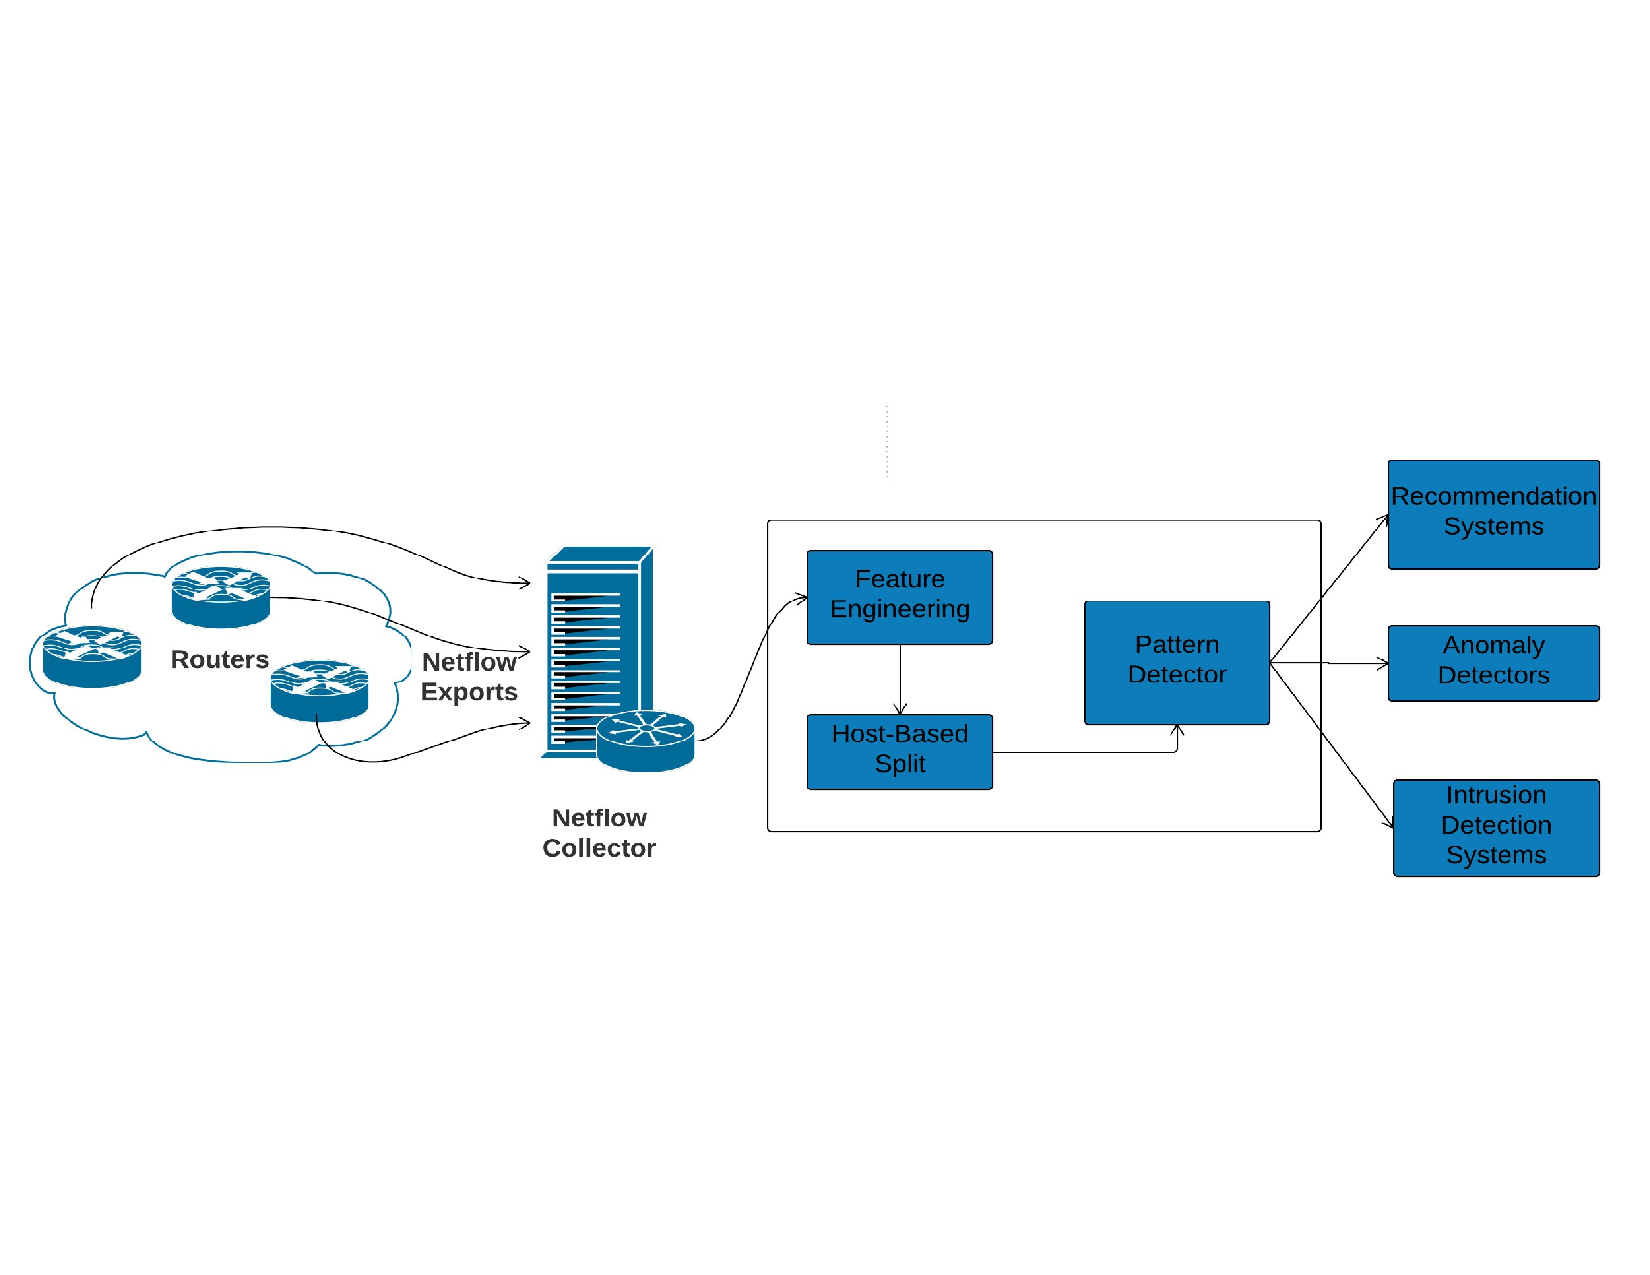
\includegraphics[trim=4cm 4cm 4cm 4cm, scale = 0.6]{architecture.pdf}}
	\caption{Architecture.}%
	\figlabel{arch}
\end{figure}

\subsection{Netflow Collection}
While the term NetFlow has become a de-facto industry standard, many other network hardware manufacturers support alternative flow technologies namely Jflow, s-flow, NetStream, etc.. The University routers from which we have collected the data for this experiment have been equipped with NetFlow on it which led to using NetFlow as our Flow technology. 
\subsubsection{What is NetFlow}
NetFlow is a proprietary protocol for collecting IP flow packets information on networks. There are different variants to this protocol but across all these versions a flow is defined uniquely by its source and destination IP addresses, source and destination ports, transportation protocol. Whenever one of these values changes a new flow is created. For each flow the number of packets, bytes and other network related information are tallied and stored in the routers cache till it expires, then this information is exported to a collector. 

The captured flows are exported to NetFlow collectors at frequent intervals. The flows that are to be exported are determined based on the following rules: 1) when it is inactive for a certain time without receiving any new packets. 2) If the flow is active than max threshold time which is configurable. 3) If a TCP flag (FIN / RST) indicates the flow is terminated. NetFlow provides a powerful tool to keep track of what kind of traffic is going on the network, and are widely used for network monitoring. Most vendors support different flavors of similar flow monitoring approaches and a common standardization is done within the IETF IPFIX working group.

There are different variants of NetFlow with each advanced version giving additional information about the flow. The fields that we used in our experiment and that are supported across the versions are in \figref{netflow}.

\begin{figure}[t]
	\centerline{
	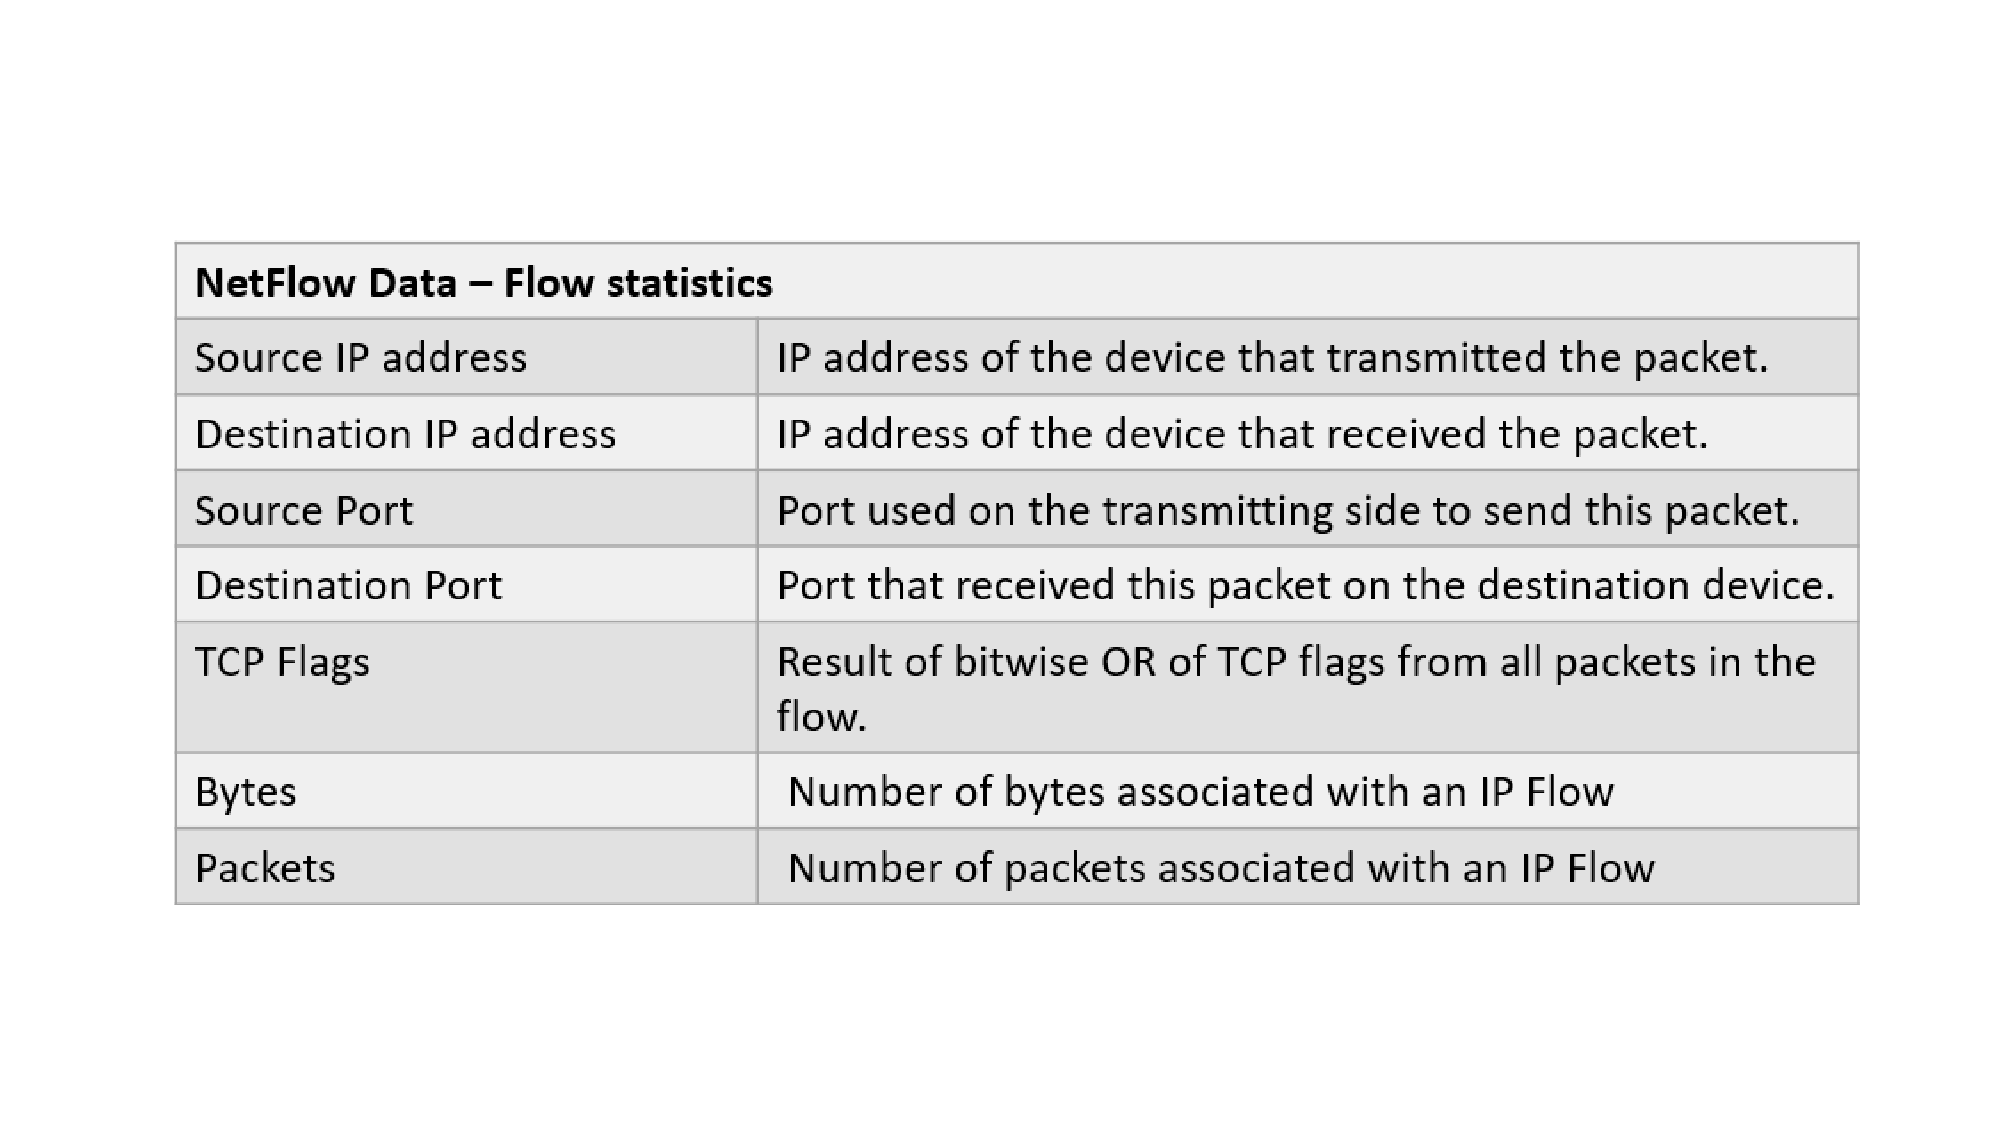
\includegraphics[trim=2cm 2cm 2cm 2cm, scale = 0.55]{netflow.pdf}}
	\caption{NetFlow Fields captured in a Flow }
	\figlabel{netflow}
\end{figure}

\subsection{Feature Engineering}

Feature Engineering is the process of transforming raw
data into features so as to better represent the underlying structure of the data. This helps in increasing the accuracy of the models we build using data mining techniques. This step comes before modeling and after seeing the data.
Features extracted from the data directly influence the models generated and predictions made out of it. The better the features are the better the results will be. The results that we achieve when we are using DM approaches are a factor of the data set in hand, the features generated , the prediction model and the way the problem is framed. Most of the times even simpler models perform better if the features describe the structure inherent to the data. 
Below we describe different steps involved in the Feature Engineering with sample set of data.
\begin{table}[t]
	\caption{Netflow raw data.}%
	\centerline{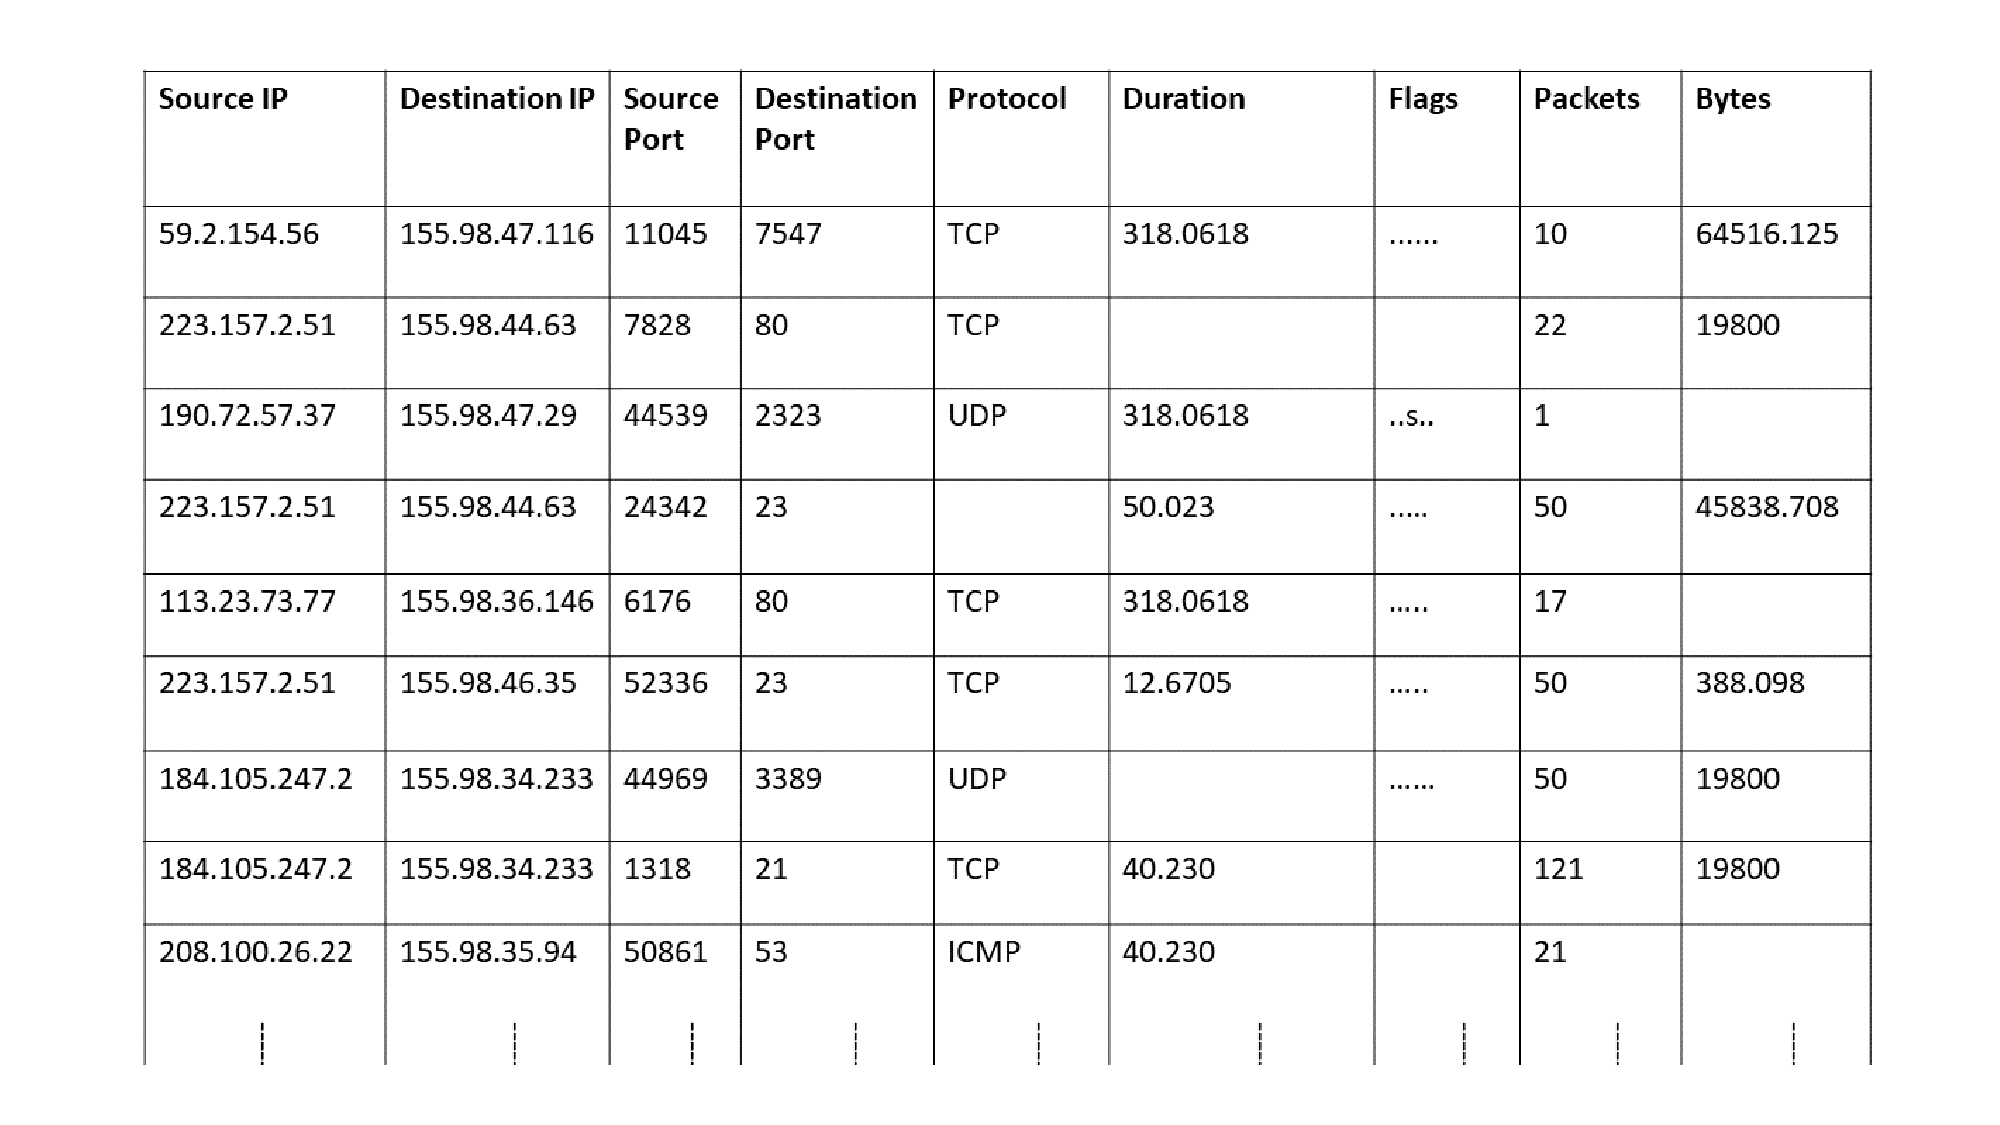
\includegraphics[scale = 0.5]{raw_data.pdf}}	
	 \tablabel{raw_data}
\end{table}
 
\subsubsection{Missing Data} 

\tabref{raw_data} is a sample of network data collected using netflow. In total there are 40 columns for each record with each column capturing different flow information. From the table we can see that there are few missing values. Missing data is a common issue that every data science experiment has to deal with and there could be different reasons why netflow records could be missing some values such as, few filters could be turned on the router that doesn't let the netflow collector collect all the information, overloading of netflow collector and others. We handled Missing data using the following techniques 

1) Replace missing values with the mean. For the features such as duration, total packets and bytes exchanged we assume that missing values are distributed similarly to the values that are present for each source IP. The rational approach here would be to substitute values using mean as it maintains the existing distribution.

2) Replace missing values with the median/ mode. This is an other technique to handle missing data, It should be noted that using different statistical measures to replace missing values yield different solutions. Features that have categorical data cannot be handled using mean or median and hence we approach mode to fill in their missing values. The feature protocols was handled using the mode approach, filling the missing values with the most frequently occurring protocol value for that source IP.

3) The question that arises when replacing missing values is what percentage of values can a feature miss atmost. For example, filling in half the values of a feature in this step with a statistic measure is not reasonable. Features of this kind are considered as noise and could affect the effectiveness of the data mining algorithm. The better option here would be to discard the coulmn that has too may missing calues. In our case there were handful of columns that fell under this category and are discarded. flags shown in the \tabref{raw_data} is one among them. After handling missing values our data looks as in \tabref{missing_data}.

\begin{table}[b]
	\caption{NetFlow raw data after handling missing values}%
	\centerline{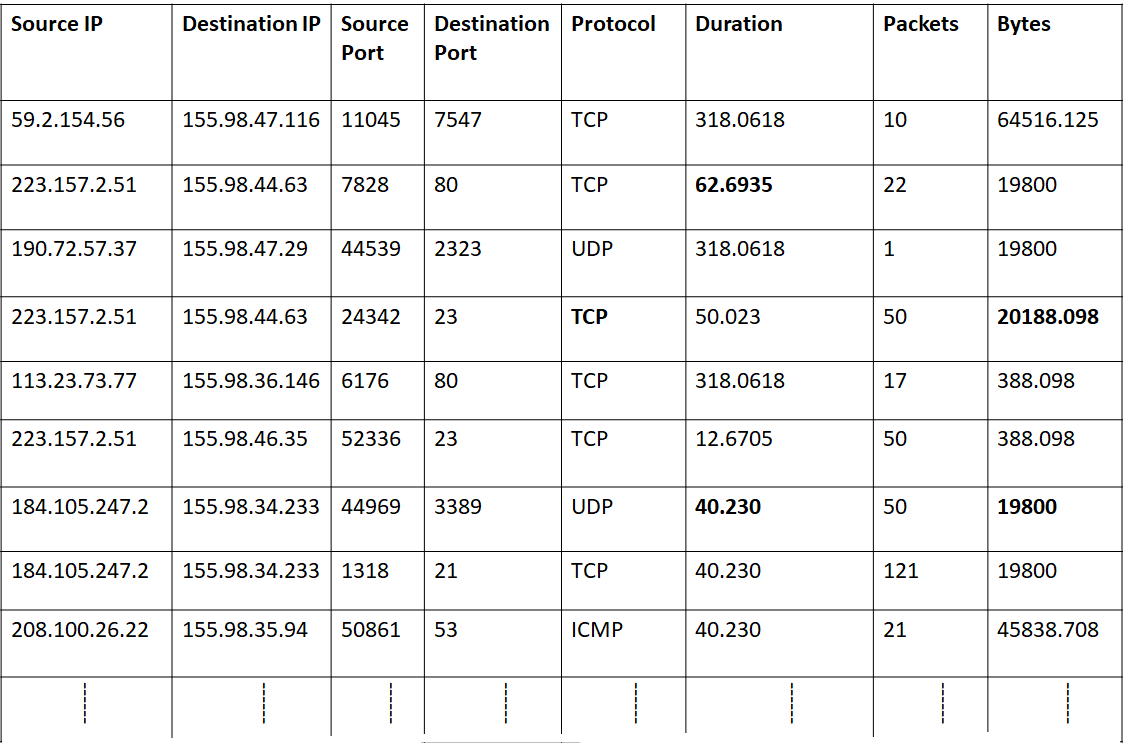
\includegraphics[scale = 0.6]{missing_data.png}}
	
	\tablabel{missing_data}
\end{table}


\subsubsection{Converting Categorical to Numerical Variables} 

Features could be either numerical or categorical variables. When dealing with algorithms that work on numerical data we have to make sure that the categorical variables are handled.
For example, in our case feature protocol, has values such as TCP, UDP and others. One approach is to encode them as 0, 1, and 2 respectively converting them to numerical variables. This could pose a problem when using distance measuring algorithms as the distance between the encoded attributes, like 1 (UDP) ,0 (TCP) is smaller than 0 (TCP) ,2 (others) generating an unintended meaning to this feature and could lead to biasing of few values. Another approach would be to create a feature for each value of the categorical variable and mark it as 0 or 1 based on if the value is present or not. There are both pros and cons to this method. The pros are if we choose to aggregate the values on all features this conversion gives a numerical value to work with. The cons are scaling and standardization could be affected. \tabref{categorical} represents data set after this step.

\begin{table}[t]
	\caption{After Converting categorical data to numerical}%
	\centerline{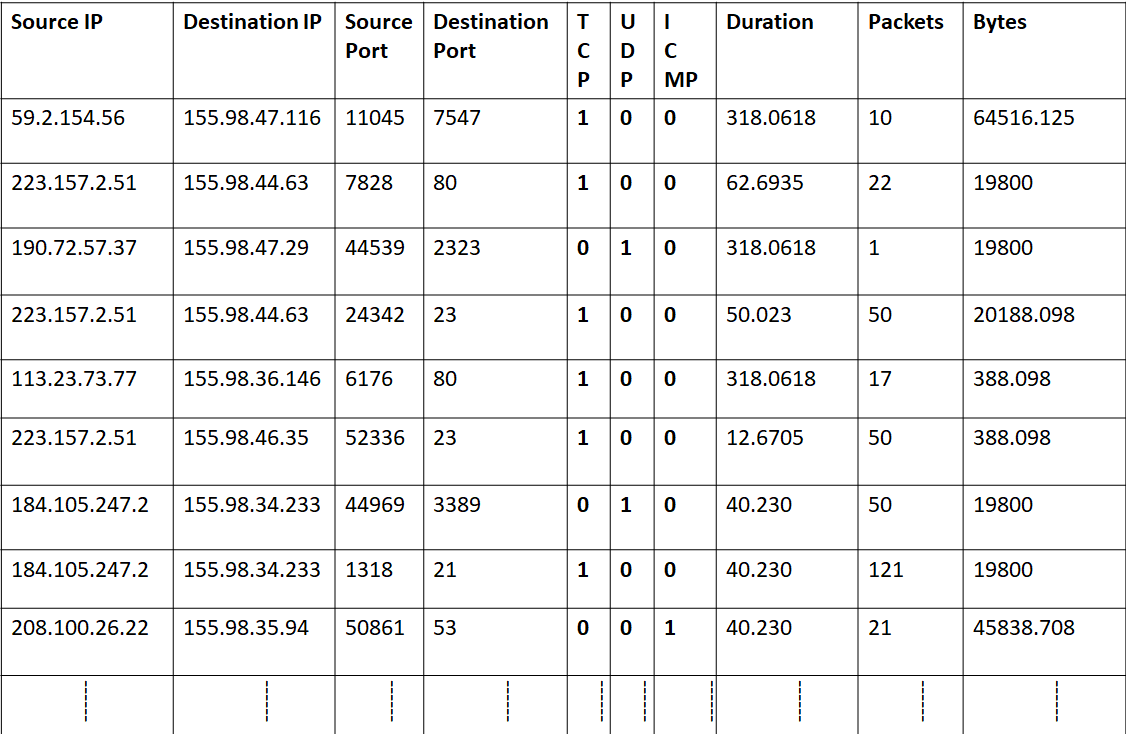
\includegraphics[scale = 0.6]{categorical.png}}
	\tablabel{categorical}
\end{table}

Above two steps fall under a family of techniques called data cleaning. After the data cleaning and removing the irrelevant columns of data using domain knowledge we aggregated netflow data based on source IP as our work focuses learning about hosts from their aggregate data. The \tabref{aggregated} shows a sample of aggregated data with ten features.
The first record in the \tabref{aggregated} conveys the information that in the given data set the host 59.2.154.56 (source IP) had appeared 450 times. Out of those 450 instances it had contacted 116 unique hosts. A total of 110 different source ports were used in the 450 flows and all the packets were sent to single destination port. The columns TCP, UDP, ICMP indicate how many of these flows fall under each category. So of the 450 flows there are 406 flows in which TCP protocol was used , 4 had UDP protocol used and the rest 40 had used ICMP protocol. And the columns Total Duration, Total Bytes, Total Packets indicate the respective information exchanged by this sourceIP on a whole. This aggregated data is what we use for learning host behaviors. But, before that we have to apply few other feature engineering techniques as described below.

\begin{table}[b]
	\caption{Aggregated data by Source IP}%
	\centerline{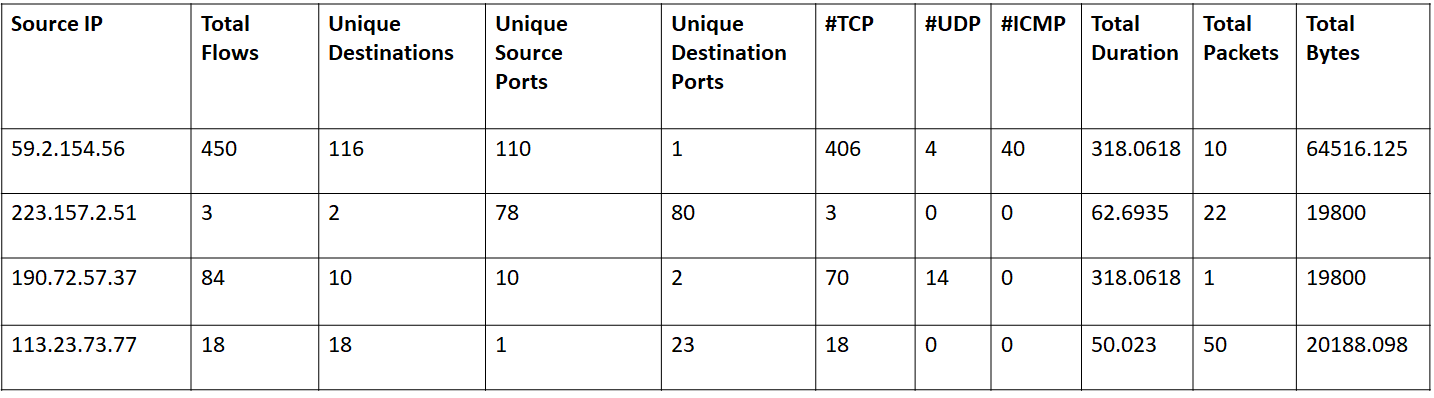
\includegraphics[scale = 0.6]{aggregated.png}}	
	\tablabel{aggregated}
\end{table}


\subsubsection{Feature Scaling} 
Feature Scaling/Feature Normalization, a method used to standardize the range of independent features of data. Failure to standardize variables might result in algorithms placing undue significance to variables that are on a higher scale. For example from the \tabref{aggregated} it is evident that the total packets and total bytes have higher magnitude compared to total flows and destinations. This range difference shouldn't bias our results.
There are different ways to do feature scaling namely, Min-Max scaling, Variance scaling, L2 normalization etc.. The choice depends on the data and different statistics of it such as Mean, Variance, L2 norm. Scaling is not advisable in all instances we might	loose valuable information if applied without proper thought. In our case we have chosen simple Min-Max scaling as our goal was merely to change the range of the data and not the distribution and Min-Max scaling helps us in achieving this at a lower cost.

\subsubsection{Feature Transformation} 
Transforming Non-normal distribution to Normal, many ML/DM tools perform well on normalized data and having skewed data will give inaccurate results. Log transformations are generally used to normalize the skewed data which is the case with most network data. After transforming the data if it doesn't capture the essence of original data we could look at other options such as square root, cube root. BoxCox is also another technique that changes the distribution of variables from non-normal to normal or near normal. \figref{feature} shows the distribution of a feature Total Flows from our aggregated data, as seen from the graph it is heavily skewed towards left and this can be directly attributed to the data set we have in hand. The graph indicates that in most instances number of flows in which a source IP appears is less than 100 and hence we employ transformation techniques to decrease the amount of skewness in the data.  \figref{feature_transformed} shows the same data after applying log transformation. 

\begin{figure}[t]
	\centerline{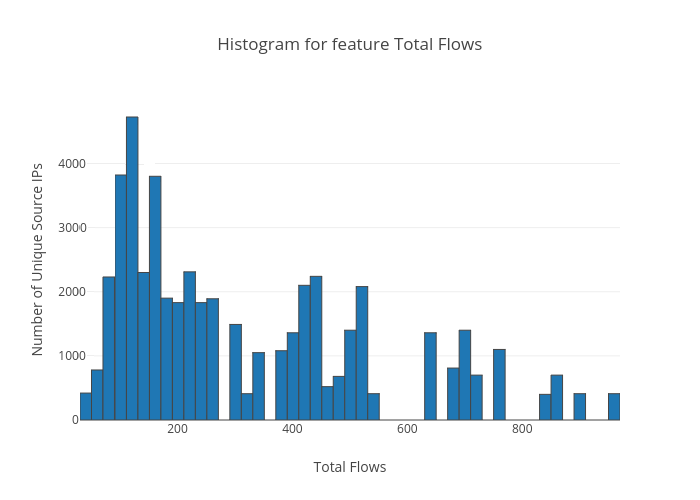
\includegraphics[scale = 0.9]{feature.png}}
	\caption{Skewed data before transformation}%
	\figlabel{feature}
\end{figure}

\begin{figure}[t]
	\centerline{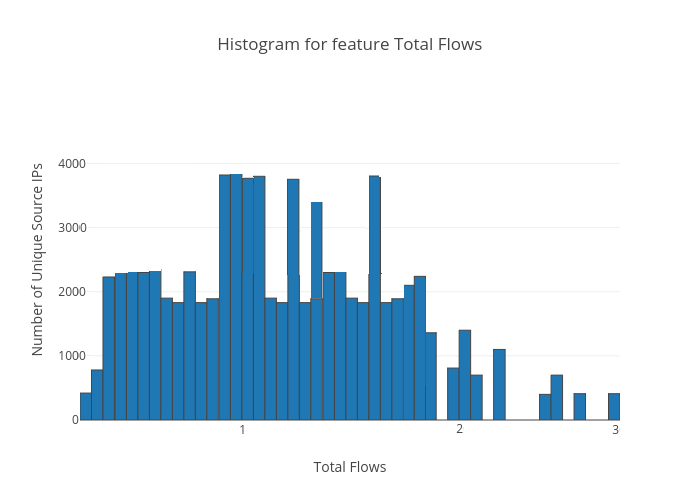
\includegraphics[scale = 0.9]{transformed.png}}
	\caption{Normalized data}%
	\figlabel{feature_transformed}
\end{figure}



\subsubsection{Feature Selection}		
	
	Feature Selection refers to the process of selecting a subset of relevant features to model the data. It helps in shorter time periods of execution, overcoming the overfitting problem and making the solution more generic and avoid curse of dimensionality. The central premise of this process is to remove redundant or irrelevant features that don't make much sense to the problem we ought to solve. Feature selection and dimensionality reduction are two confusing terms. Though, both methods seek to reduce the number of attributes in the dataset, but dimensionality reduction does it by creating new combinations of attributes, where as feature selection methods include and exclude attributes present in the data without changing them. Principal Component Analysis, Singular Value Decomposition are examples of dimensionality reduction methods. The techniques used to do feature selection depend on text, numerical variables and they are three general classes of them Filter, Wrapper, Embedded methods.	Feature selection is a much tougher problem in unsupervised setting as we don't have any labels that helpus in determining the information gain with and without a feature.Problems of
	this kind have been rarely studied in the literature \cite{boutsidis2009unsupervised} \cite{dash2002feature}. 
	
	The common strategy of most approaches is the use of filter methods Filter model methods do not utilize any clustering algorithm to test the quality of the features. They evaluate the score of each feature according to criteria \cite{dash2002feature} mentioned here. It selects the features with the highest score. It is called the filter since it filters out the irrelevant features using given criteria. 
	Wrapper methods are an other class of methods used for feature selection where we train the given model with different combinations of features and make inferences accordingly.
	Some common examples of wrapper methods are forward feature selection, backward feature elimination and recursive feature elimination. Forward selection is similar to elbow method explained in the next section. It is an iterative technique where we start with zero features and in each step we keep adding feature that has the most information gain or best expresses the underlying structure. This procedure is stopped when addition of an extra feature doesn't add any significant information to the model. forward The backward eliminaion technique is exactly opposite to the Forward selection method. Here we start with all the features and remove the least significant feature at each iteration. This iterative procedure stops when no improvement is observed on removal of features.
	
	We have chosen wrapper methods backward elimination technique for feature selection as it measures the usefulness of a subset of features by actually training a model on it. Though, it is computationally expensive compared to Filter based approaches in our context it was reasonable as we had only 10 features to look into. The result of feature selection is we have detected two features that have very less information gain namely the ICMP ports and duration and hence we removed these two from our feature list making our final feature count to 8.
	 Feature Selection has helped us in enabling the machine learning algorithm to train faster. It reduced the complexity of the model and made it easier to interpret. We were also able to address the overfitting problem.






\section{Pattern Detector}
Pattern Detector consists of the core logic of our system. After cleaning the data and applying feature engineering we send the data through a pattern detector. Pattern Detector sends the data through a clustering algorithm. It then maps the generated clusters to the host behaviors which is explained later.

As mentioned in the background section we choose to address our problem using unsupervised learning approaches. The most common unsupervised learning method is cluster analysis, which is used for exploratory data analysis to find hidden patterns or grouping in data. 

\subsubsection*{Why K-Means ??}
 In the section \ref{unsupervised} we have discussed about different type of clustering techniques in detail. Here we provide a reasoning for choosing K-Means.
 
Connectivity models like Hierarchical clustering don't have a provision for relocating objects that may have been incorrectly grouped at an early stage. Also, use of different distance metrics for measuring distances between clusters may generate different results. Performing multiple experiments and comparing
the results is recommended to support the veracity of
the original results. Lastly, Time complexity of at least O($n^2logn$) is required, where n is the number of data points thus lacking scalability for handling big datasets.

Distribution Models assume a distribution for data but for many real data sets, there may be no concisely defined mathematical model (e.g. assuming Gaussian distributions is a rather strong assumption on the data). Also, though distribution models have an excellent  theoretical foundation but they suffer from one key problem known as overfitting. 

We have experimented our data set with the density model DBSCAN and we have found the data being grouped at most in to only two clusters. The reason for this is that density based models expect some kind of density drop to detect cluster borders. Recall from the above section that our data set has many source IPs that appear in less than 100 flows and hence there wasn't any drop in density observed resulting in bad clustering.

Experimenting with centroid models especially K-Means gave us an advantage to play with the variable K and view into how host behaviors are being grouped with different values of K. It is scalable for heavier datasets and doesn't suffer from the overfitting problem. Also, there isn't any inherent assumption on which distribution the dataset should follow. Thus, making it a clear choice for building our system.


\subsubsection*{How to choose K ??}
 In many situations, parameters and variables chosen by the algorithm or by users affects the performance of the algorithm differently and results in different outputs. Similarly, an essential problem of the K-means clustering method is to define an appropriate number of clusters K. In the literature there are different approaches proposed to determine an accurate value of K.
 These methods include direct methods and statistical testing methods. Direct methods consists of optimizing a criterion, such as the within cluster sums of squares or the average silhouette. The corresponding methods are named elbow and silhouette methods, respectively. Statistical testing methods consists of comparing evidence against null hypothesis. An example is the gap statistic. We have used the direct methods as they optimize a criteria the elbow method to determine K and then cross-verified the values with the Silhouette Index obtained for this same data set.
 
 Recall that, the basic idea behind partitioning methods, such as k-means clustering, is to define clusters such that the total intra-cluster variation [or total within-cluster sum of square (WSS)] is minimized. The total WSS measures the compactness of the clustering and we want it to be as small as possible. The Elbow method looks at the total WSS as a function of the number of clusters: One should choose a number of clusters so that adding another cluster doesn’t improve much better the total WSS. 
 The optimal number of clusters can be defined as follow:
 \begin{itemize}
 	\item Compute k-means clustering for different values of k. For instance, by varying k from 1 to 50 clusters.
 	
 	\item For each k, calculate the total within-cluster sum of square ($W_k$).
 	\begin{center}
 	 	\boldsymbol{$D_k = \sum_{x_i \in C_k} \sum_{x_j \in C_k} ||{x_i -x_j}||^2$}	 \\
 	 	
 	 	
 	 	\boldsymbol{$ W_k = \sum_{1}^{K} \frac{1}{n_k} D_k$}
 	\end{center}  
    Where K is the number of clusters, $n_k$ is the number of points in cluster k and $D_k$ is the sum of distances between all points in the cluster.
 	\item Plot the curve of wss according to the number of clusters k. 	
 	\item The location of a bend (knee) in the plot is generally considered as an indicator of the appropriate number of clusters.
 \end{itemize}

 	The graph depicts the amount of information we are gaining with addition of each cluster. the first clusters will add much information, but at some point the marginal gain will drop, giving an angle in the graph. The number of clusters are chosen at this point, hence the elbow criterion. \figref{elbow} shows the elbow curve obtained for our data set on a chosen day. This method gave us a value of 7 for K.
 	

\begin{figure}[t]
	\centerline{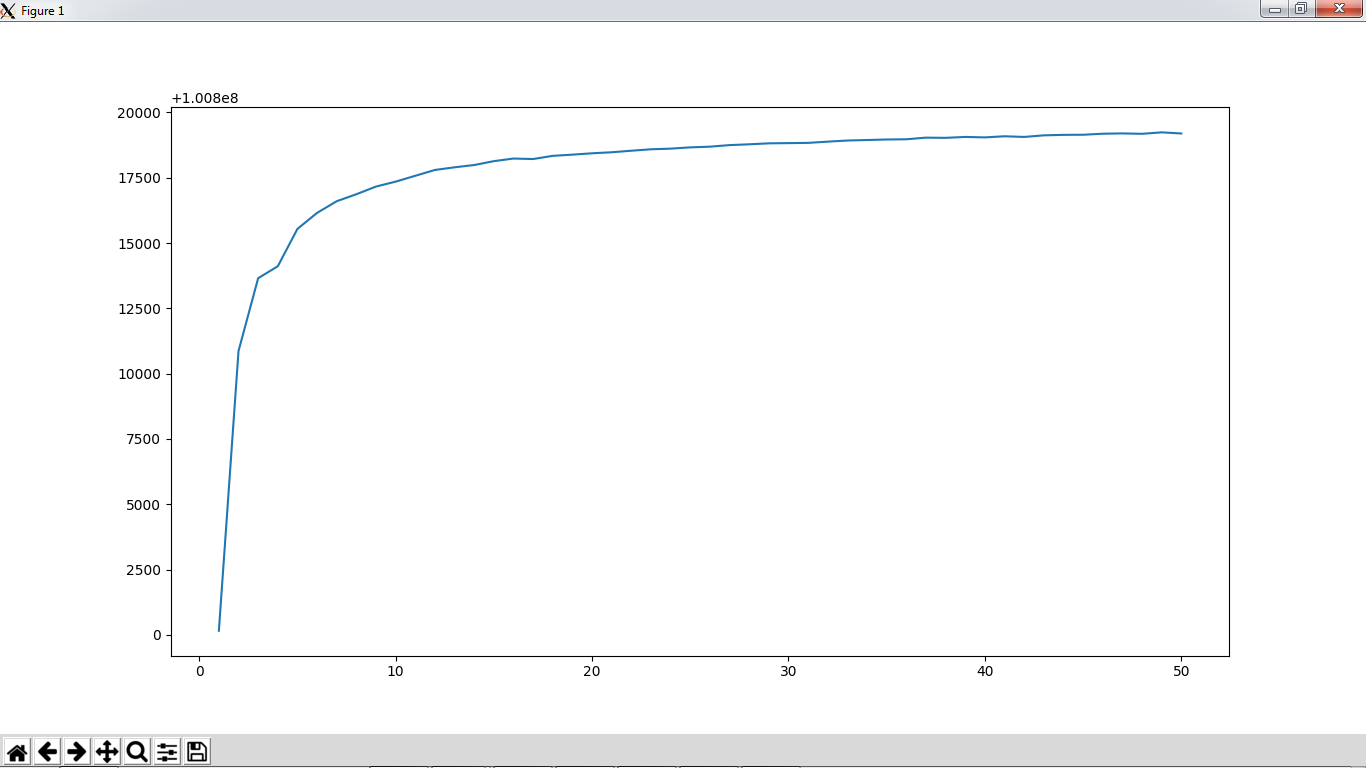
\includegraphics[scale = 0.4]{elbow.png}}
	\caption{Elbow Method}%
	\figlabel{elbow}
\end{figure}

 However, the elbow method is not unambiguous. especially if the data is not very clustered we will notice that the elbow chart will not have a clear elbow. Instead, we see a fairly smooth curve, and it's unclear what is the best value of k to choose. In cases like this, we might try a different method for determining the optimal k. Hence, to corroborate the claim of elbow method for K we also ran our data set through another technique called silhouette.

	The average silhouette approach measures the quality of a clustering. That is, it determines how well each object lies within its cluster. A high average silhouette width indicates a good clustering.	Average silhouette method computes the average silhouette of observations for different values of k. The optimal number of clusters k is the one that maximize the average silhouette over a range of possible values for k.	The algorithm is similar to the elbow method and can be computed as follow: 
	
	\begin{itemize}
		\item Compute k-means clustering for different values of k. For instance, by varying k from 1 to 50 clusters.
		\item For each k, calculate the average silhouette of observations (avg.sil).
		
		\begin{center}
			\boldsymbol{$s(i) = \frac{b(i) - a(i)}{max(a(i),b(i))}$}
		\end{center}
		Here s(i) is the silhouette index of a cluster point i. Where a(i) is the average distance of point i to all the objects in the same cluster while b(i) is the minimum average distance from the point i to all the points of different cluster. avg.sil is calculated by finding mean of all the s(i) for each point in a cluster.
		
		\item Plot the curve of avg.sil according to the number of clusters k.
		\item The location of the maximum is considered as the appropriate number of clusters.
	\end{itemize}
 
  The intuition behind this approach is for a point as a(i) is a measure of how dissimilar i is to its own cluster, a small value means it is well matched. Furthermore, a large b(i) implies that i is badly matched to its neighboring cluster. Thus an s(i) close to one means that the data is appropriately clustered. if s(i) is close to negative one, then by the same logic we see that i would be more appropriate if it was clustered in its neighboring cluster. The average s(i) over all data of a cluster is a measure of how tightly grouped all the data in the cluster are. Thus the average s(i) over all data of the entire dataset is a measure of how appropriately the data have been clustered. \figref{silhouette} shows the the plot obtained using silhouette technique. 
 
 \begin{figure}[t]
 	\centerline{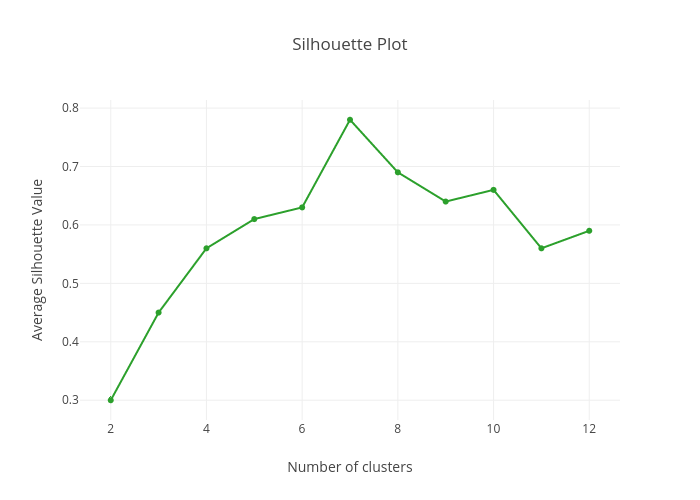
\includegraphics[scale = 0.6]{silhouette.png}}
 	\caption{Silhouette Method}%
 	\figlabel{silhouette}
 \end{figure}
 
\subsubsection*{Cluster Labeling}  \label{cluster_labeling}

We chose a reference day for labeling the clusters. Since the number of clusters are only seven we had manually inspected each cluster and labeled them based on the contents of the cluster. \tabref{cluster_centers} shows clusters formed and the cluster centers. The first row describes that the cluster 1 has hosts which on an average sent 10 outgoing flows by using 9 different source ports targeting a single destination on the same port and all those flows were UDP flows. 

We have mapped each of these clusters to human understandable classes which is shown in \tabref{cluster_label}. The clusters represent the host behaviors as follows:

\begin{itemize}
	\item Cluster 1 represents hosts which are sending DNS queries to our servers and they are classified as Low as they have an average of 10 flows. 
	
	\item Cluster 2 hosts exchange normal tcp traffic. These hosts could various things ranging from exchanging messages to files.
	
	\item Cluster 4 represents the hosts similar to the Cluster 1 hosts which are sending DNS queries to our servers and they are classified as high as they have an average of 200 flows.
	
	\item Cluster 3 and Cluster 5 represent to the Heavy and Low DNS Query Responses. The hosts in these clusters correspond to Heavy and Low DNS queries respectively.
	
	\item Cluster 7 represents only UDP flows.
	
	\item Cluster 6 represents anomalous hosts trying to scan through the network  by sending heavy packets or trying to gain unauthorized access through open ports. 
\end{itemize}

\begin{table}[b]
	\caption{Cluster Centers}%
	\centerline{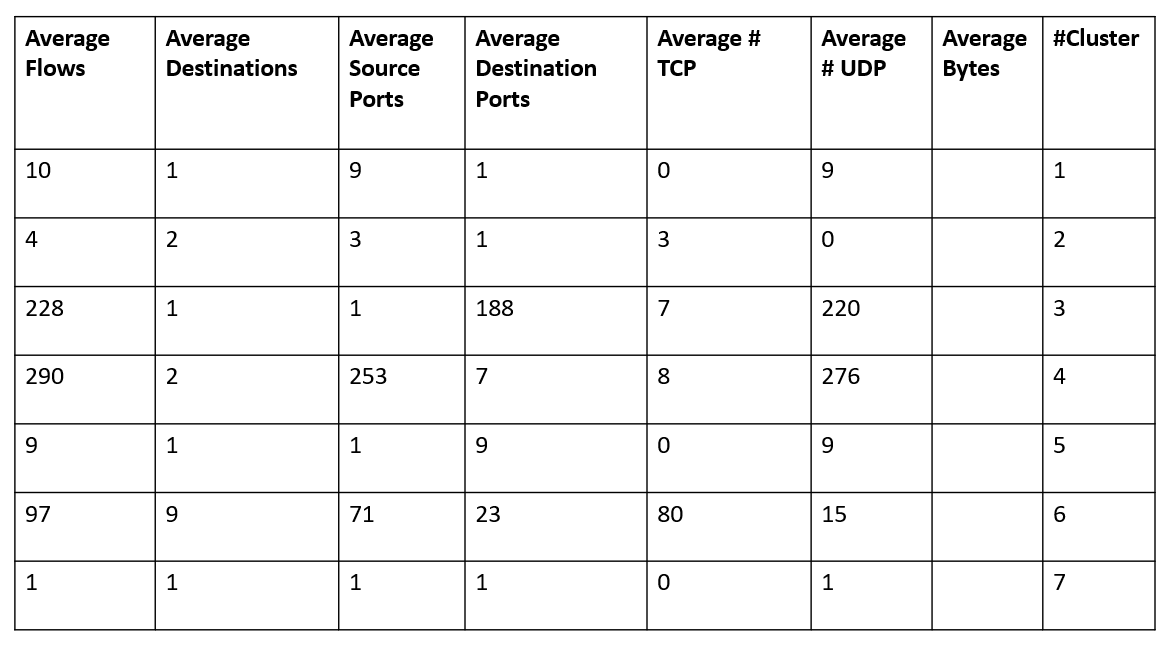
\includegraphics[scale = 0.6]{cluster_centers.png}}
	
	\tablabel{cluster_centers}
\end{table}

\begin{table}[b]
		\caption{Cluster Labeling}%
	\centerline{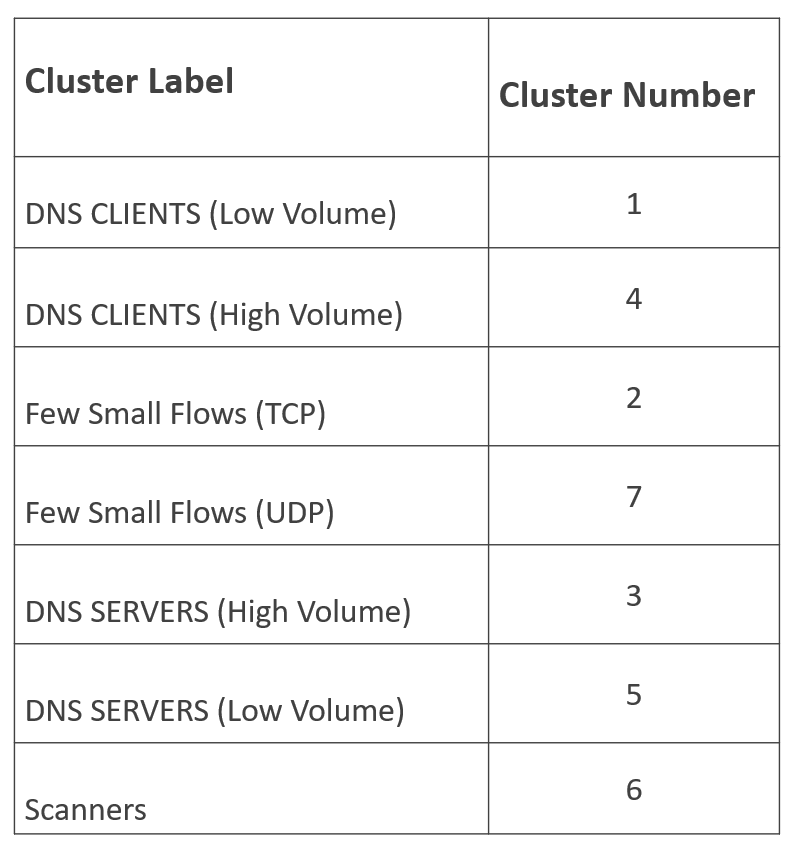
\includegraphics[scale = 0.6]{cluster_label.png}}

	\tablabel{cluster_label}
\end{table}

\subsubsection*{Cluster Comparison}
As mentioned the overarching premise of our work is to analyze the behavior of hosts looking at the aggregated data. In order to analyze the behavior of hosts over a time period we should be able to compare hosts behavior across days. We dealt with this by initially comparing the hosts behavior for any two days and then extended it to any given time period.

In our case each cluster is exhibiting a unique behavior and hence comparing the hosts behavior turns out to be a problem of comparing clusters formed on two different days. Cluster comparison is not a well studied area. And, hence we translated this problem into an Assignment problem \cite{kuhn1955hungarian}. Assignment problem is a special type of linear programming problem which deals with the allocation of the various resources to the various activities on one to one basis. It does it in such a way that the cost or time involved in the process is minimum and profit or sale is maximum. 

In our case both the resources and activities are nothing but clusters formed on two different days. Assignment Problem is a well studied problem and has polynomial time solutions. One such algorithm is the Hungarian algorithm. 

\section{Applications}
Our system can be used to build different applciations that help in Network Management. Few of them are as follows:
\textit{Recommendation Systems}, We can capture the different behaviors exhibited by network users over time and use this to predict a behavior on a certain day of a week or month using the historical data. This helps network admin to prepare well ahead and plan the bandwidth or other network resources accordingly.
\textit{Recommendation Systems}, We can capture the different behaviors exhibited by network users over time and use this to predict a behavior on a certain day of a week or month using the historical data. This helps network admin to prepare well ahead and plan the bandwidth or other network resources accordingly.
\textit{Recommendation Systems}, We can capture the different behaviors exhibited by network users over time and use this to predict a behavior on a certain day of a week or month using the historical data. This helps network admin to prepare well ahead and plan the bandwidth or other network resources accordingly.

%In that direction of building a recommendation system we came up with an user interface that helps to analyze historic data , this should go into evaluation section.%



